%A pesar de que Manticore permita el uso de valores simbólicos para el parámetro \texttt{(msg.sender)} las limitaciones de la herramienta exigen que se defina cada account individualmente para que sea considerada en el estado de la blockchain.
Las limitaciones de la herramienta exigen que el parámetro \texttt{(msg.sender)}, a pesar de que pueda ser simbólico, se corresponda con una \textit{account} definida explícitamente por el usuario.
Por esto en la simulación contamos con un número fijo de \textit{accounts}, asignando variables simbólicas únicamente la información asociada a ellas (Dirección, Balance, etc).

\section{Comparación de las abstracciones generadas entre el algoritmo clásico y el alternativo}
Como mencionamos en la sección \ref{sec:subaproximacion}, las abstracciones generadas por el algoritmo alternativo no siempre son Enabledness Preserving Abstractions\footnote{Es decir, en algunos casos no cumplen la definición presentada en la sección \ref{definicion-epa}.} de los contratos analizados, sino que son unas subaproximaciones de estas.
Al mismo tiempo, las EPAs son sobreaproximaciones del comportamiento de los contratos, por lo que el mecanismo resultante del algoritmo alternativo yace en algún lugar intermedio: no es ni sound ni complete.
Por esto, nos interesa explorar en particular cuáles son las diferencias producidas entre el algoritmo alternativo y las generadas por el algoritmo clásico (las EPAs) para evaluar su utilidad.
Para responder estas preguntas analizamos el desempeño de los prototipos implementados usando ambos algoritmos sobre algunos casos de prueba.

\subsection{Caso \texttt{RoomThermostat}}
El primer caso que evaluamos fue el contrato \texttt{RoomThermostat} perteneciente al benchmark ``Microsoft Azure Blockchain Workbench" \cite{azure-benchmark}, cuyo código fuente podemos ver en la figura \ref{fig:rooomthermostat-solidity}.
Es un contrato pequeño, con pocos métodos y un invariante sencillo.
Para poder emplear el algoritmo clásico sobre este contrato, el invariante propuesto fue el siguiente:
\begin{lstlisting}[language=Solidity]
    function invariant(StateType stateNew, address installerNew, address userNew, int targetTemperatureNew, ModeEnum modeNew) public returns(bool){
        bool result = (stateNew == StateType.Created || stateNew == StateType.InUse);
        result = result && (modeNew == ModeEnum.Auto || modeNew == ModeEnum.Cool || modeNew == ModeEnum.Heat || modeNew == ModeEnum.Off);
        if(stateNew == StateType.Created){
            result = (targetTemperatureNew == 70) && (modeNew == ModeEnum.Off);
        }
        return result;
    }
\end{lstlisting}

Luego, evaluamos tanto el algoritmo clásico como el alternativo sobre el contrato.
En ambos casos la EPA generada fue la misma, una máquina de estados sencilla de tan sólo tres estados que podemos ver en la figura \ref{fig:room-thermostat-epa}.

\begin{figure}
    \centering
    \begin{subfigure}{0.75\textwidth}
        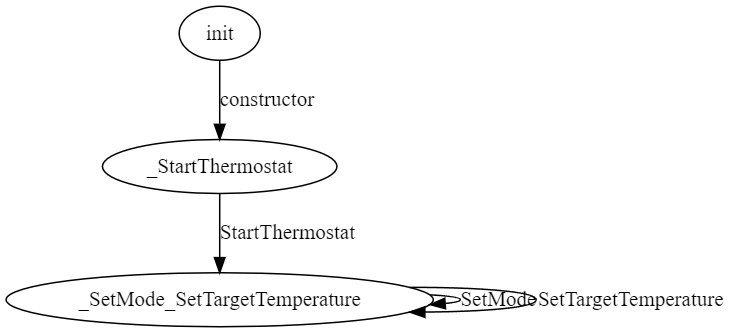
\includegraphics[width=\textwidth]{figs/room-thermostate-epa.png}
        \caption{Enabledness Preserving Abstraction del contrato \texttt{RoomThermostat} }
        \label{fig:room-thermostat-epa}
    \end{subfigure}
\end{figure}

\subsection{Caso \texttt{BoundedStack}}
El siguiente caso que evaluamos fue el ejemplo teórico que expusimos en la sección \ref{sec:subaproximacion}, el contrato \texttt{BoundedStack}, con intención de evidenciar las subaproximaiones realizadas por el algoritmo nuevo.
El código del contrato se encuentra en la imagen \ref{code:solidity-bounded-stack}.
Nos interesa corroborar el comportamiento de ambos algoritmos, si se produce alguna subaproximación, y cuáles.

Lo primero que vimos al evaluar la abstracción generada por el algoritmo alternativo sobre el contrato \texttt{BoundedStack} lo podemos ver en la imagen \ref{fig:buggy-bounded-stack-epa}.
En esa abstracción  podemos ver que faltan algunas de las transiciones presentes en la EPA del contrato, pero además podemos observar que las transiciones por \textcolor{orange}{\texttt{pop}} siempre llevan al estado desde el que se ejecutó el método.
Cuando realizamos esta comparación generó bastante confusión, hasta que comprendimos que se debía a un error en el código fuente de \texttt{BoundedStack} que no decrementaba la variable \texttt{size} al ejecutar \textcolor{orange}{\texttt{pop}}.
Luego de corregir el error, la abstracción generada por el prototipo fue la referenciada en la imagen \ref{fig:bounded-stack-bad-epa}.
Es decir, la misma que elaboramos durante el ejemplo teórico del comportamiento del algoritmo alternativo.
Decidimos incluir este pequeña caso de un error en el código fuente en lugar de omitirlo para ejemplificar que, a pesar de que quede evidenciado que el algoritmo nuevo genere subaproximaciones de las EPAs en la práctica, las abstracciones generadas pueden seguir resultando útiles a la hora de atrapar errores.

\begin{figure}[H]
    \centering
    \begin{subfigure}{0.45\textwidth}
        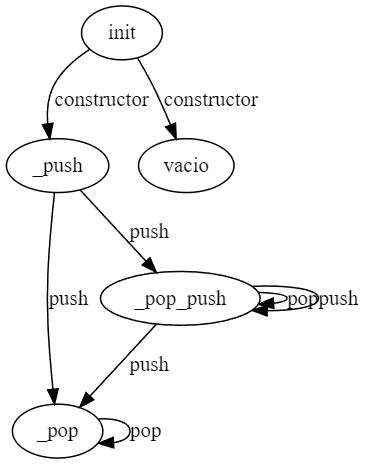
\includegraphics[width=\textwidth]{figs/buggy-bounded-stack-epa.png}
        \caption{Enabledness Preserving Abstraction del contrato \texttt{BoundedStack} con un error que no decrementa el tamaño luego de ejecutar \textcolor{orange}{\texttt{pop}} }
        \label{fig:buggy-bounded-stack-epa}
    \end{subfigure}
\end{figure}

A la hora de emplear el algoritmo clásico sobre el contrato, el invariante propuesto fue el siguiente:
\begin{lstlisting}[language=Solidity]
    function invariant() public returns(bool){
        bool result = (size >= 0) && (size <= maxSize);
        result = result && (internal_arr.length == size);
        return result;
    }
\end{lstlisting}

Sin embargo, el prototipo desarrollado con el algoritmo clásico no pudo analizar este contrato satisfactoriamente, sino que terminó el analisis por time out.
Esto se debe a que el paso de restringir las instancias del contrato a aquellas que satisfagan el invariante resultó demasiado difícil para el motor de ejecucion simbólica de Manticore
Algunos experimentos y análisis intermedios nos hacen creer que se debe a la pobre representación de las variables de tipo \textcolor{cyan}{\texttt{uint256[]}} del mismo.
Esto significó que terminamos el análisis comparando la abstracción generada por el algoritmo alternativo no con la generada por el algoritmo clásico, sino con una EPA producida manualmente.

\section{Comparación en tiempo de ejecución entre el algoritmo clásico y el alternativo}
Otra hipótesis generada durante el desarrollo del algoritmo alternativo fue que el evitar la ejecución de los invariantes mejoraría el tiempo de ejecución.
Esto se debe a que son propiedades relativamente complejas, comparadas con las precondiciones de los métodos externos, que pueden predicar sobre el estado de variables internas de tipos complejos como arrays, mappings, etc.
Para evaluar esta hipótesis estudiamos el tiempo de ejecución empleado por los prototipos que implementan el algoritmo alternativo y el clásico en Manticore sobre algunos de los contratos pertenecientes al benchmark Microsoft Azure Blockchain Workbench \cite{azure-benchmark}.

Ya que este mismo benchmark había sido utilizado por Godoy et al. en 2022 \cite{predicate-abstraction-for-smart-contract-validation}, a la hora de experimentar contamos con EPAs de todos los contratos involucrados, lo que pudimos usar para corroborar la correctitud de las abstracciones generadas.
Para realizar el análisis, ejecutamos ambos prototipos sobre cada contrato cinco veces en una máquina \textbf{DESCRIPCION MAQUINA} y tomamos el promedio del tiempo empleado.

En la figura \ref{fig:classic-vs-alternativo} podemos ver

\begin{figure}
    \centering
    \begin{subfigure}{0.65\textwidth}
        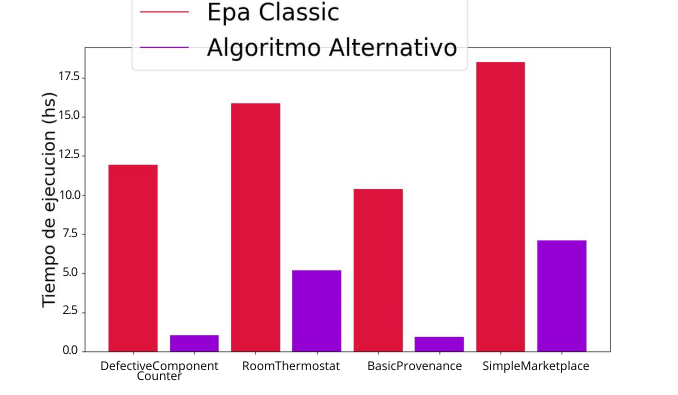
\includegraphics[width=\textwidth]{figs/classic_vs_alternativo.png}
        \caption{Tiempo de ejecución (en promedio) de la generación de abstracciones del prototipo que implementa el algoritmo alternativo y el algoritmo clásico}
        \label{fig:classic-vs-alternativo}
    \end{subfigure}
\end{figure}
Al evaluar el funcionamiento del prototipo buscamos responder las siguientes preguntas:
\begin{enumerate}
    \item ¿Son correctas las EPAs que genera el prototipo?
    \item ¿Cuál es su performance en contratos inteligentes reales?
\end{enumerate}
Para responder estas preguntas, pusimos el prototipo a prueba contra algunos contratos provenientes de Microsoft Azure Blockchain Workbench \cite{azure-benchmark}.
Este conjunto de contratos había sido utilizado anteriormente por Godoy et al. \cite{predicate-abstraction-for-smart-contract-validation}, por lo que convenientemente ya contamos con las EPAs correspondientes.
Ejecutamos el prototipo cinco veces, obteniendo el promedio de su tiempo de ejecución sobre los contratos seleccionados y luego corroboramos que la EPA generada fuera isomórfica a la obtenida en los estudios anteriores.
%Además, pusimos a prueba la cantidad de accounts necesarias para el funcionamiento del prototipo.
Los resultados intermedios indicaron que para los contratos propuestos era suficiente realizar la simulación con dos \textit{accounts}, por lo que utilizamos esa cantidad para los experimentos.
Los resultados de esta experimentación se ven resumidos en la tabla \ref{tab:resultados}.
El prototipo generó EPAs correctas en todos los casos.
Sin embargo, el tiempo de cálculo es de entre media y casi tres horas, considerando incluso que los ejemplos utilizados son relativmente pequeños.
Algunos resultados intermedios indican que este tiempo es consumido principalmente por Manticore para la generación de \textit{path conditions}.
Debido a la rigurosidad con la que emula Manticore el comportamiento de la blockchain, la herramienta demora incluso para la ejecución simbólica de transiciones sencillas.

\vspace{-2.2em}

\begin{table}
    %\begin{adjustwidth}{-0.5in}{-0.5in}% adjust the L and R margins by 1 inch
    \caption{Resumen de la experimentación. \textbf{LOC} es cantidad de lineas de código, \textbf{Tiempo de ejecución} es el promedio del tiempo de ejecución medido en minutos, $\boldsymbol{\sigma}$ es el desvío estandard medido en segundos y \textbf{¿Es correcto?} indica si la EPA generada es isomorfa con la provista anteriormente.}\label{tab:resultados}
    \begin{tabular}{|l|l|l|l|l|}
        \hline
        Contrato                  & LOC & Tiempo de ejecución (min) & $\sigma$ (s) & ¿Es correcto? \\
        \hline
        DefectiveComponentCounter & 33  & $29$                      & $7$          & Sí            \\
        SimpleMarketplace         & 66  & $186$                     & $800$        & Sí            \\
        BasicProvenance           & 48  & $40$                      & $6$          & Sí            \\
        RoomThermostat            & 48  & $138$                     & $600$        & Sí            \\
        \hline
    \end{tabular}
    %\end{adjustwidth}
\end{table}
